% This is a sample document using the University of Minnesota, Morris, Computer Science
% Senior Seminar modification of the ACM sig-alternate style. Much of this content is taken
% directly from the ACM sample document illustrating the use of the sig-alternate class. Certain
% parts that we never use have been removed to simplify the example, and a few additional
% components have been added.

% See https://github.com/UMM-CSci/Senior_seminar_templates for more info and to make
% suggestions and corrections.

\documentclass{sig-alternate}
\usepackage{color}
\usepackage[colorinlistoftodos]{todonotes}
\usepackage{comment}
\usepackage{amsmath}
\usepackage{hyperref}
\usepackage[linesnumbered,ruled,vlined]{algorithm2e}
\hypersetup{
    colorlinks=true,
    linkcolor=black,
    filecolor=black,      
    urlcolor=cyan,
    citecolor=black
}

%%%%% Uncomment the following line and comment out the previous one
%%%%% to remove all comments
%%%%% NOTE: comments still occupy a line even if invisible;
%%%%% Don't write them as a separate paragraph
%\newcommand{\mycomment}[1]{}

\begin{document}

% --- Author Metadata here ---
%%% REMEMBER TO CHANGE THE SEMESTER AND YEAR AS NEEDED
\conferenceinfo{UMM CSci Senior Seminar Conference, April 2019}{Morris, MN}

\title{Wing Design Using SAIL}

\numberofauthors{1}

\author{
% The command \alignauthor (no curly braces needed) should
% precede each author name, affiliation/snail-mail address and
% e-mail address. Additionally, tag each line of
% affiliation/address with \affaddr, and tag the
% e-mail address with \email.
\alignauthor
Leonid Scott\\
	\affaddr{Division of Science and Mathematics}\\
	\affaddr{University of Minnesota, Morris}\\
	\affaddr{Morris, Minnesota, USA 56267}\\
	\email{scot0530@morris.umn.edu}
}

\maketitle
\begin{abstract}
In engineering spaces where modeling is difficult, engineers seek a variety of well performing solutions in order to concentrate resources on promising areas of the problem space. 
We call this process \textit{illumination}.
Gaire et al have designed an algorithm specifically for illumination of problem spaces where the underlying model is computationally expensive.
This algorithm, Surrogate Assisted Illumination (SAIL) uses an \textit{evolutionary algorithm} called MAP-Elites to do illumination.
However, SAIL introduces a Gaussian process to simulate the computationally expensive model, and bayesian optimization for quality control of the Gaussian process.
SAIL has demonstrated potential for finding a variety of well performing solutions when applied to the design of aerodynamic hulls for \textit{velomobiles}.
We will walk through each of the components of the SAIL algorithm, and the results of the velomobile experiment. 

\begin{comment}
This paper takes a deep dive into Gaier et al's paper, \textit{Data-Efficient Design Exploration through Surrogate-Assisted Illumination}.
While many evolutionary algorithms attempt to find the optimal solution to a problem space, Gaier et al develops an evolutionary algorithm that \textit{illuminates} the problem space. 
This concept is particularly attractive in aerospace engineering as it allows engineers to properly survey the possible landscape of wing designs before investing into one particular concept heavily.

Gaier et al build off of the work of a previous algorithm called \textit{MAP-Elites}. 
MAP-Elites is designed to provide a number of high performing solutions that represent diverse regions of performance from the problem space. 
Experiments in Monet et al show MAP-Elites to be effective in creating this diverse set of solutions.
However, MAP-Elites has been shown to be extremely computationally expensive.
Moreover, MAP-Elites relies on a static model that does not change during an evolutionary run.

Gaier et al set out to improve MAP-Elites in the context of problem spaces where:
 \begin{enumerate}
   \item Running a high fidelity model is too computationally expensive to run per individual created.
   \item Running each generation comes at a significant computational cost and accuracy cost.
 \end{enumerate}
Gaier et al's algorithm, SAIL (Surrogate Assisted Illumination), uses a surrogate model to approximate the fitness of a solution instead of high fidelity model.
In its current implementation, SAIL uses a Gaussian process as a surrogate model. In order to guess where to select new individuals, SAIL uses Bayesian Optimization (BO).
BO allows SAIL to reduce the number of generations it needs to acquire a strong, diverse set of solutions that represent a problem space well. 

This paper conducts two different experiments to test SAIL's viability in the context of aerospace engineering.
The first test attempts to design a set of two dimensional airfoils. A second test was added to design the three dimensional shape of a velomobile.
This second test was deemed important as the model to test it was much more complicated than its two dimensional counterpart.
This difficult model would stress SAIL's Surrogate Assisted model to a greater extent.
\end{comment}
\end{abstract}

\keywords{Evolutionary Computation, MAP-Elites, Gausian Processes, Bayesian Optimization}

\section{Introduction}
\label{sec:introduction}

Fluid dynamics stands as one of the most difficult problem spaces to model and thus design in.
The equations that govern fluid flow, known as the \textit{Navier-Stokes equations}, are a set of of partial differential equations with no known solution.
As a result, aerospace engineers must use extraordinary computational power to approximate Navier-Stokes results.
High fidelity models of aerodynamic devices can take hours to simulate and still impart noticeable error.
Given the difficulty in modeling fluid flow, designing wing shapes is an extraordinary challenge.

Optimization tools aid in this challenge by helping engineers at the end of the design cycle by refining a design to what is known as a \textit{local optima}.
In difficult problem spaces such as fluid dynamics, there is no guarantee that an optimizer has found the best possible solution across the entire problem space.
However, the optimizer can be very confident that it has found the best solution in one small region.
We call the optimal solution across the entire problem space a \textit{global optima}, and an optimal solution in a subsection of the problem space a \textit{local optima}. 

In 2014, Autodesk, a producer of modelling and optimizing software found that their software was being used in a peculiar way by engineers.
Instead of using optimizing tools at the end of the design process to refine designs, engineers used them at the beginning to explore the space of possible designs\cite{Bradner:2014:PTD:2664323.2664349}.
Instead of using these tools to find, with great accuracy, one local optima, they were used to find several local optima throughout the problem space.
By finding several local optima, designers could see what tradeoffs are inherent in the problem space, and hone in on regions of interest.
This process is known as \textit{illumination}.

Over the course of several years, a research group consisting of Adam Gaier, Alexander Asteroth, and Jean-Baptiste Mouret have developed a purpose built algorithm to illuminate problem spaces, particularly when models are computationally expensive.
This algorithm, known as \textit{Surrogate-Assisted Illumination} (SAIL) uses a thus far reliable method for exploring problem spaces known as evolutionary computation, albeit in a very specialized form.
The goal of SAIL is to produce a series of high performing solutions, across the problem space, to challenging engineering problems.

\section{Evolutionary Algorithms}
\label{sec:evolutionaryAlgorithms}

SAIL uses a type of \emph{evolutionary algorithm} (EA) to explore and exploit the problem space.
Evolutionary algorithms are stochastic algorithms (algorithms including randomness) inspired by biological evolution.
The premise of an evolutionary algorithm is that a population of potential solutions is tested against a model of the problem and assigned a \textit{fitness score}.
The individuals with the best fitness scores move onto the next generation and produce ``offspring''.
Over many generations the performance against the model will improve until a target performance is obtained, or the algorithm reaches a fixed number of generations. 

\begin{figure*}[th]
\centering
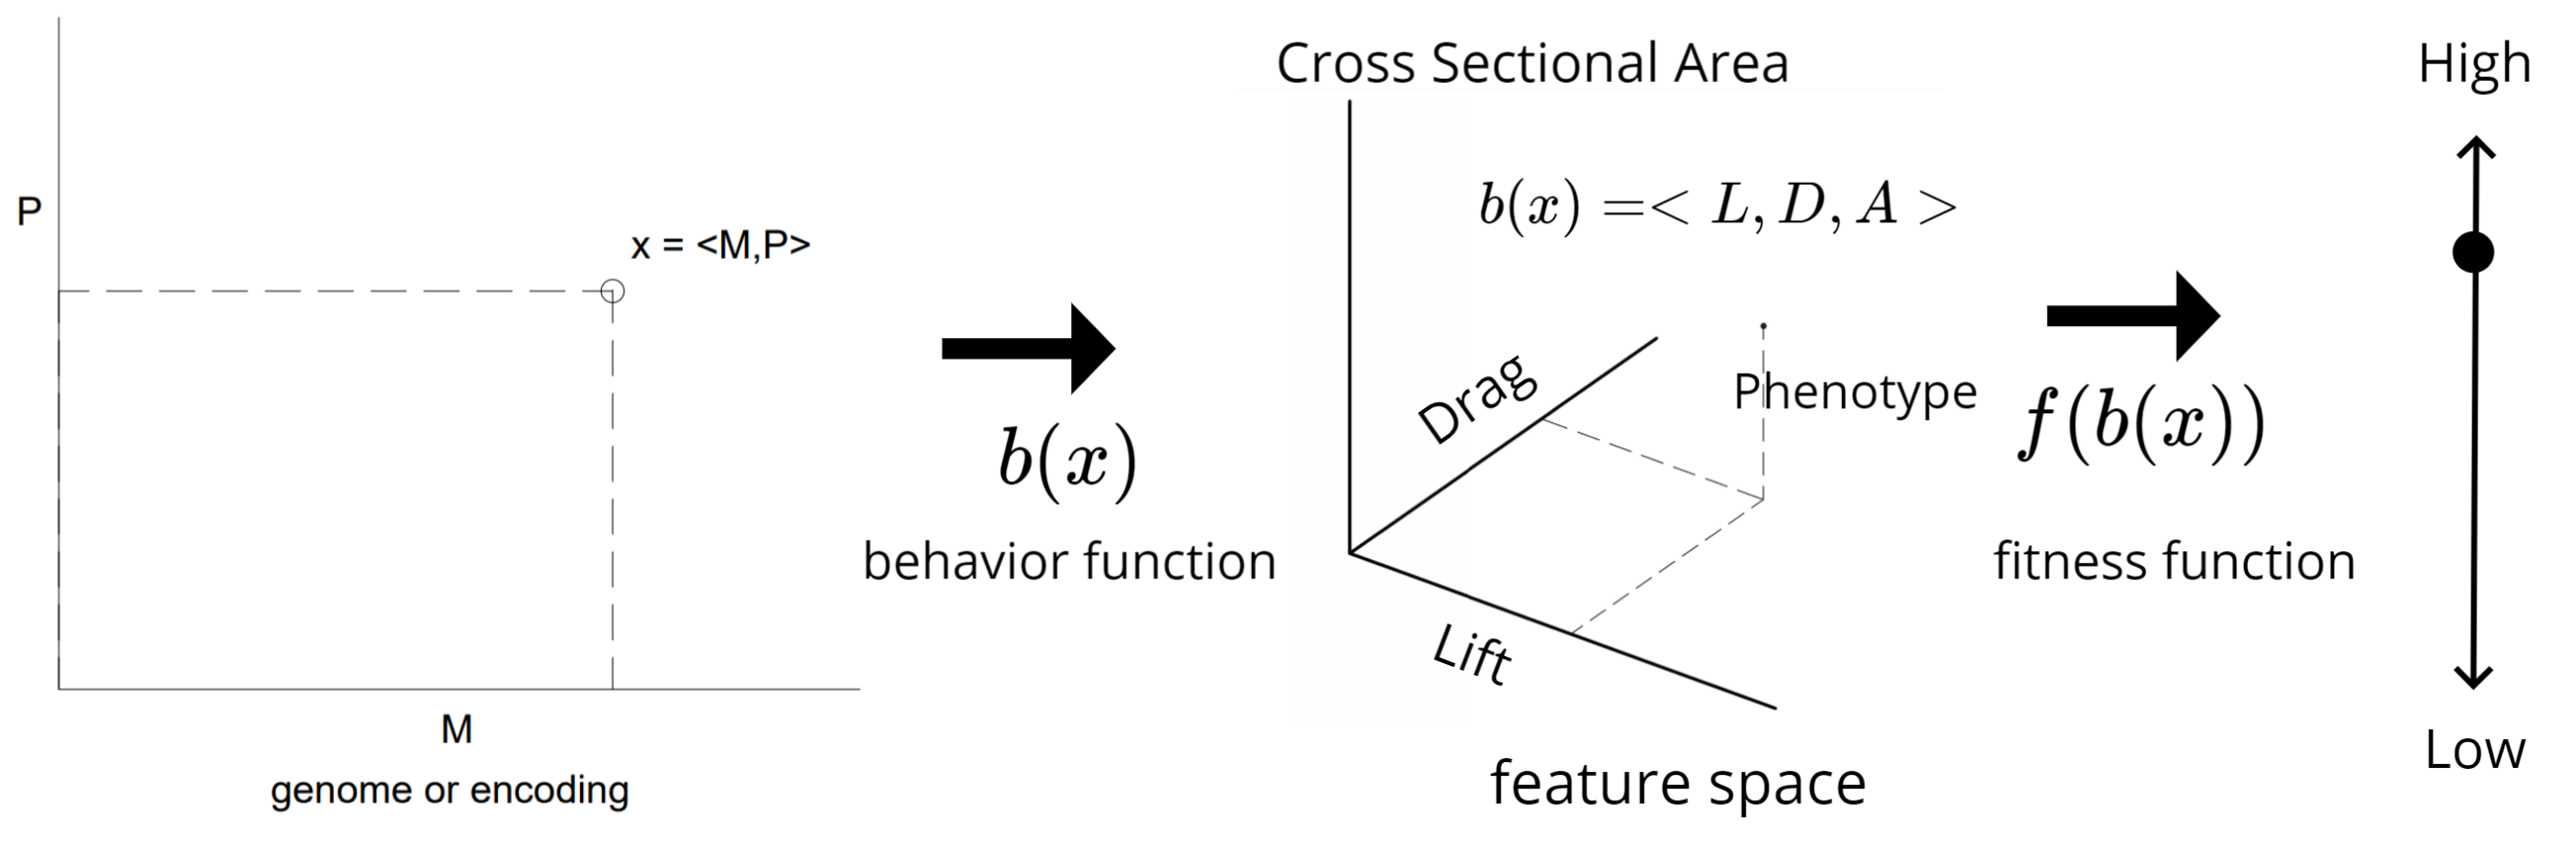
\psfig{file=CycleOfLife.PNG,width=\textwidth}
\caption{Process of moving from an individual genome to a fitness score.}
\label{fig:genome-to-fitness}
\end{figure*}

\section{SAIL Architecture}
\label{sec:SAILBuildUp}
SAIL is made up of three major components:
MAP-Elites is the evolutionary algorithm that illuminates problem spaces.
Gaussian processes approximate the computationally expensive model.
Finally, bayesian optimization enforces quality control of the Gaussian process.
This section will explain each of these components in depth before constructing Surrogate Assisted Illumination.

\subsection{MAP-Elites}
\label{sec:MAP-Elites}

MAP-Elites is an evolutionary algorithm developed in April 2015 by Jean-Baptiste Mouret and Jeff Clune~\cite{Mouret:2015}.
The purpose of MAP-Elites is to \textit{illuminate} the problem space.
That is, to produce a series of high performing solutions that represent different trade offs and insights into the problem space.
Before moving into the details of MAP-Elites, it is important to understand the terminology surrounding individuals in MAP-Elites (See Figure \ref{fig:genome-to-fitness}).

\subsubsection{Genotypes}
\label{sec:genotypes}

An important aspect in the application of any evolutionary algorithm is the way that individuals are represented.
In engineering contexts, there is a need to represent a physical object in all of its complexities in a compact and understandable form.
In evolutionary algorithms, this representation is referred to as an \textit{encoding} or a \textit{genotype} interchangeably.
For example, a common way to represent a two dimensional \textit{foil} (wing shape) is with a format called the NACA 4 Digit Series \cite{wiki:NACAairfoil}.
NACA 4 digit foils contain three numbers refering to important geometric features of the foil shape, but also directly relate to foil performance.

\begin{figure}[htb]
\centering
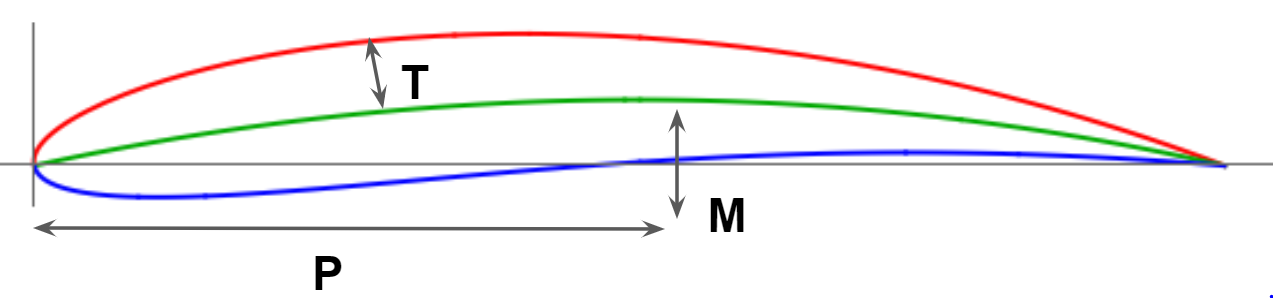
\psfig{file=NACA4-Desc.PNG,width = 3in}
\caption{Description of NACA 4 Foil.}
\label{fig:NACA4}
\end{figure}

Figure \ref{fig:NACA4} describes these three values geometrically:
$M$ refers to how ``arched'' the foil is.
$P$ describes where the most ``arched'' part of the foil exists.
Finally, $T$, refers to the thickness of the foil at its thickest point. 
Figure \ref{fig:genome-to-fitness} shows a \textit{solutions space}, the space of all genomes.
In this example, we hold thickness constant so the solution space is in two dimensions.
With this compact genotype for a 2D foil, it is possible to represent a large range of complex shapes with only three numbers.

\subsubsection{Phenotypes}
\label{sec:phenotypes}

Once we have a representation of an individual, we can start deriving its \textit{behaviors}, or \textit{phenotypes}.
In this example, those behaviors are the \emph{lift} and \emph{drag} of the foil in a certain fluid condition as well as \emph{cross-sectional area} (the space between the top and bottom lines in Figure \ref{fig:NACA4}).
In Figure \ref{fig:genome-to-fitness}, the \textit{feature space}, the space of all possible phenotypes, will exist in three dimensions: lift, drag, and cross-sectional area.
The function that takes in an individual and returns its phenotype is known as the \textit{behavior function}, $b(x)$.

\subsubsection{Fitness}
\label{sec:fitness}

MAP-Elites requires some sort of specific score so that it can definitively tell that one foil is ``better'' than another.
The \textit{fitness function} $f(x)$, takes an individual and its behaviors and returns a score quantifying how well it accomplishes our specified goals.
When developing a foil shape, we most certainly care about lift and drag, but for weight and structural reasons, we might also care about the foil's cross-sectional area.
A fitness function that encompasses these behaviors into a single score might look like this:
$$f(x) = a*\textit{Lift}(x) - b *\textit{Drag}(x) - c*\textit{Area}(x)$$
where $a$, $b$, and $c$ are constants defined by the engineer based on which factors are more important than others.
Heree, $f(x)$ is setup such that a \textit{higher} fitness score means a foil is better at achieving our goals, but it doesn't have to be that way.
Fitness functions can be setup such that a good score is a: small score, a small absolute value, etc...

\subsubsection{MAP-Elites}

MAP-Elites works by discretizing the feature space into a set of bins.
Each bin in the grid represents tradeoffs between features.
For example, the feature space in Figure \ref{fig:FeatureSpace} is split into three sections per dimension, with three dimensions, this results in 27 bins in the feature space.
The highlighted box indicates individuals with high lift, medium drag, and medium cross sectional area.

Each generation in MAP-Elites begins by creating an individual from the search space and computing its behaviors using the behavior function.
The results of the behavior function will place it in a bin of the feature space.
If there is already an individual in that bin, the fitness function will be computed on both individuals, and the individual with the superior fitness will end that generation occupying the bin.
If there is no individual in that bin, the new individual simply occupies it.

In the initial generation (generation 0), a randomly generated population of individuals is created from the search space.
Those individuals then compete for spots in the feature space.
The individuals who occupy a bin at the end of a generation are known as \textit{elites}.
During each subsequent generation, a new individual is randomly generated.
That new individual will compete with the elites from the previous generation for a bin in the feature space.

\begin{figure}[tb]
\centering
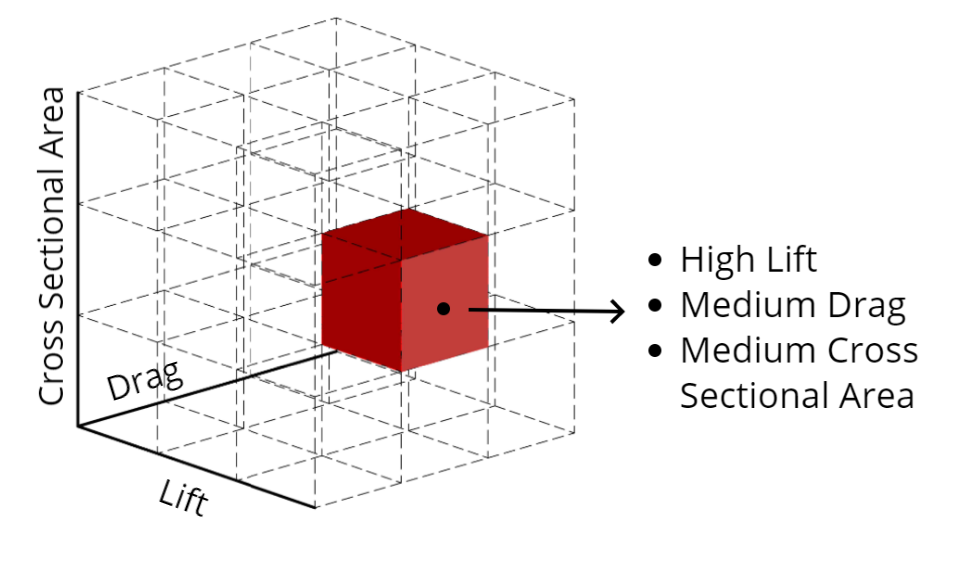
\psfig{file=DiscretizedSpace.PNG,width = 3in}
\caption{How MAP-Elites disrectizes a feature space. Here, each of three dimensions is split into three sections, yielding 27 ``bins''.}
\label{fig:FeatureSpace}
\end{figure}

By default, MAP-Elites creates new individuals by choosing a random elite and ``tweaking'' it.
This process is called \textit{mutation}.
Because small changes in the genome of an individual can result in large changes in behavior, it is common for the mutated individual to compete in a different bin than the parent.

The designer can decide how MAP-Elites terminates.
Termination can happen  after:
A fixed number of generations or computational cost is exceeded.
One or many elites have a fitness over a given threshold.
Alternatively, after a certain number of bins are filled.


The last point alludes to an important aspect of MAP-Elites: not all bins can always be filled.
In our example, physics does not allow a foil to have high lift, zero drag, and minimal cross-sectional area.
For this reason, the highest lift, lowest drag, lowest cross-sectional area bin might not be filled.
In addition to finding good solutions for a problem, MAP-Elites also offers insights on just where the physics of a problem caps performance of solutions.

\label{MAPElitesSub}

\subsection{Gaussian Process}
\label{gaussianProcess}
Like many evolutionary algorithms, MAP-Elites evaluates the model's fitness and behavior functions several times per generation.
Considering a single MAP-Elites run can involve hundreds of thousands, or even millions of generations, the model needs to be computationally inexpensive.
However, in engineering contexts like fluid dynamics, computing lift and drag of a foil in high fidelity can take hours.
In these cases, the model is prohibitively computationally expensive for use in traditional evolutionary algorithms.

SAIL avoids computing the model directly most of the time by utilizing \textit{surrogate models} to approximate the model.
Surrogate models strategically execute the model in only limited points of the problem space.
They then use this information to extrapolate what other parts of the model should behave like.
Gaier et al have chosen to use \textit{Gaussian processes} (GPs) as a surrogate model because they require very few queries from the model in order to start extrapolating from the problem space.
In addition, GP's include information about how confident they are about the extrapolation of a certain point in the problem space.

%\begin{figure}[htb]
%\centering
%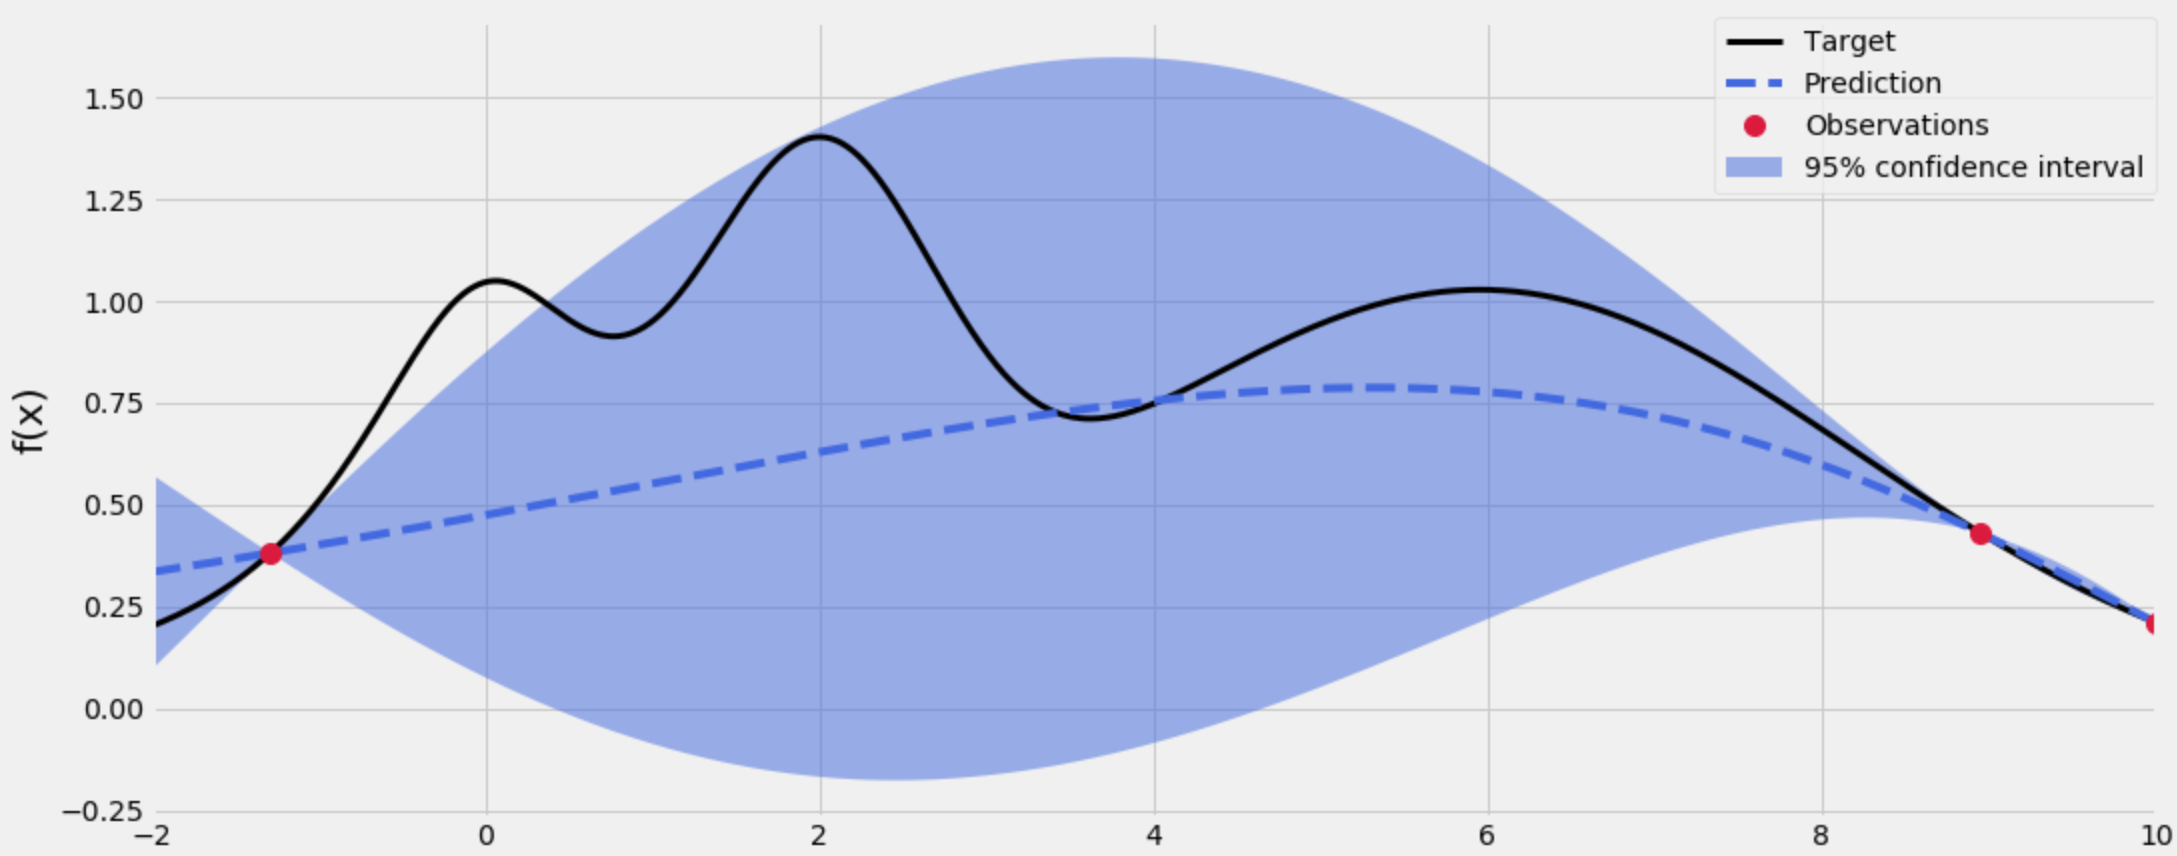
\psfig{file=GP-T3.PNG,width = 3in}
%\label{fig:GPT3}
%\caption{The plot of a Gaussian processes trying to model a %function $f(x)$ with three observed values (There is an observed %value on the far right).}
%\end{figure}

Space constraints limit us from diving into the statistics driving Gaussian processes.
Instead, we will walk through how they are used.\footnote{If you would like to learn the mechanics behind Gaussian processes, Dr. Nando de Freitas has a fantastic set of recorded lectures:
\url{https://youtu.be/4vGiHC35j9s}
}
Figure \ref{fig:BO5} shows a Gaussian process that is trying to model a target function shown in black.
The GP has four observed points to build its model from (shown as red dots in figure \ref{fig:BO5}).
With these observations, the GP can begin to extrapolate what a value of $f(x_{*})$ might be for a given $x_{*}$.
The GP will return a prediction, and a confidence in its extrapolation of $f(x_{*})$.

If we extrapolate a large number of points, to the degree in which they blend together to look like lines, we get Figure \ref{fig:BO5}.
The GP prediction for each of these extrapolations form the blue dashed line.
We call this dashed line, the \textit{mean prediction} of the Gaussian process.
The confidence at each extrapolation blends into two lines:
upper and lower confidence intervals.
These confidence bounds define the top and bottom of the GP prediction the figure.
The confidence bounds in Figure \ref{fig:BO5} are drawn such that we are 95\% certain that the true value of $f(x_{*})$ is within these bounds.
Moreover, for each extrapolated $x_{*}$, we are most confident that the true value of $f(x_{*})$ is on the mean prediction line.
From there, the likelihood of the true value of $f(x_{*})$ drops off with distance from the mean prediction line.

Areas that have low confidence, and a wide spread are said to have \textit{high variance}.
The variance contracts around our observed points, and expands as we get farther away from the observed points.
This leads to an important feature of Gaussian processes:
\textit{Where there is data, we are confident, where there is no data, we are less confident}.

\subsection{Bayesian Optimization}
\label{bayesianOptimization}

The fact that Gaussian processes are confident where there is data, and less confident where there is not, allows us to ask an important question:
\textit{If we were to add another point to our Gaussian process, where would we do it?}
If our objective is to maximize the function modeled by our Gaussian processes in Figure \ref{fig:BO5}, then our new point can help us do that in one of two ways:
First, we could try to pick a point where our prediction is maximized,near $x=5$; this is called \textit{exploiting} our problem space.
Second, there are two areas between $x=0$ to $x=2$ and $x=5$ to $x=7$ with high variance.
Selecting a point in this area would improve the overall accuracy of our model, and there might just be a maxima to our function in that region.
Selecting a point for this rational is called \textit{exploring} the problem space.

\begin{figure}[htb]
\centering
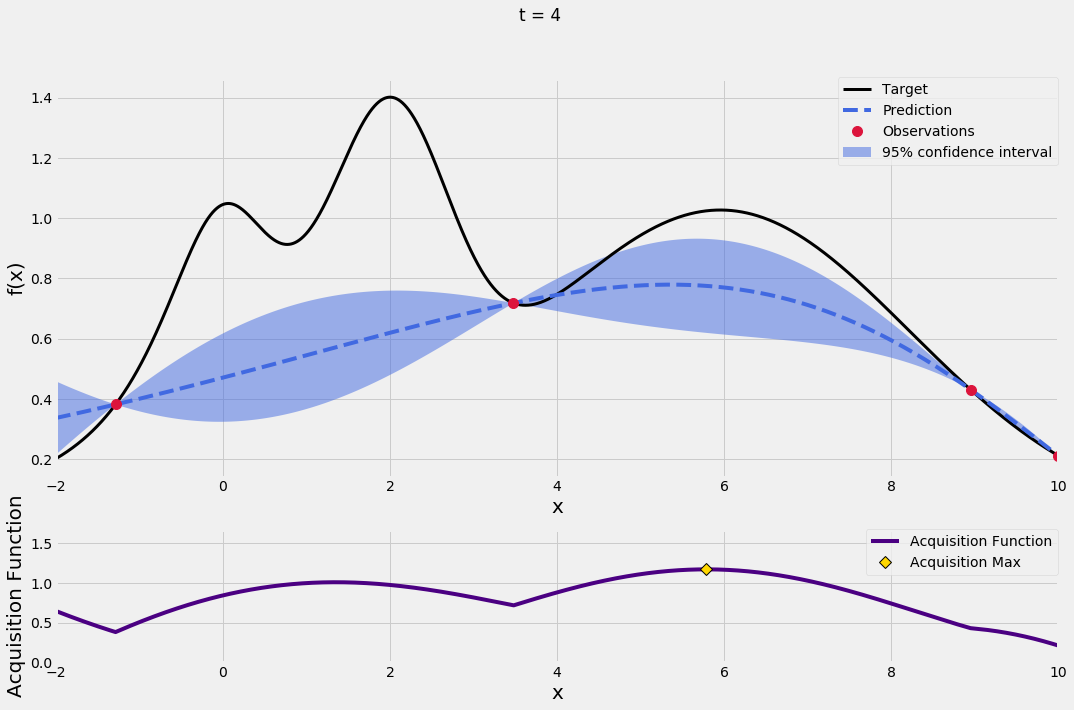
\psfig{file=t-4.png,width = 3in}
\label{fig:t4}
\end{figure}

\begin{figure}[htb]
\centering
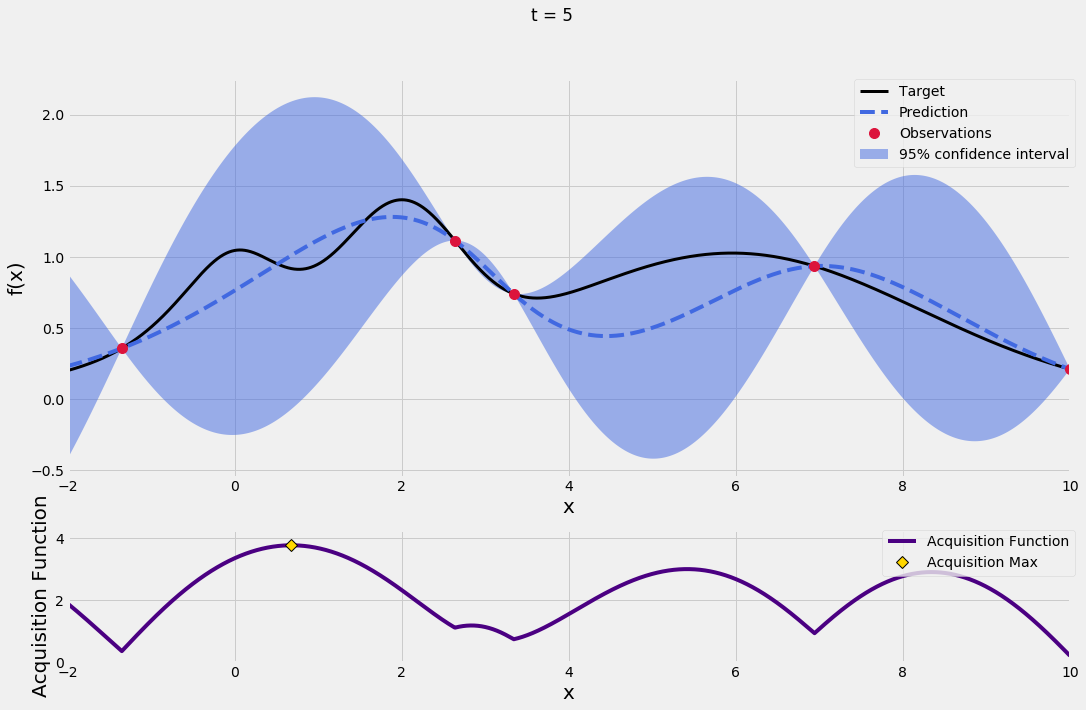
\psfig{file=t-5.png,width = 3in}
\caption{A Gaussian processes modelling a function $f(x)$ with four points (top image), and five points on the bottom.
One of the observed values is on the far right.
For both GP's, the UCB acquisition function is computed in purple.
Taken from \cite{rand:BayesianOptimization}}
\label{fig:BO5}
\end{figure}

The degree to which we should explore or exploit the problem space is a difficult question.
\textit{Bayesian optimization} attempts to balance these objectives by providing a rule for computing the utility of observing another point.
There are many different ways of computing utility with bayesian optimization;
Gair et al decided to use the \textit{Upper Confidence Bound Optimizer}:

\[ UCB(x) = \mu(x) + k\sigma(x) \]

The utility of observing a new value from the model, the $UCB(x)$ at a point $x$, is the linear combination of the the mean prediction at a point, $\mu(x)$, and some constant $k$, times the variance, $\sigma(x)$, at some point.
Varying $k$ tunes the model to favor exploration vs exploitation in different quantities. We call the resulting function the \textit{acquisition function}.

Figure \ref{fig:BO5} shows how a bayesian optimization is applied to a Gaussian processes.
The UCB, in purple, is computed along the x axis.
The top image shows the GP with four observations.
At this stage, the model is not doing too well at approximating the true function.
Maximizing the acquisition function gives us a point with both a high approximated value and a high variance. 

We select that point, re-compute the Gaussian processes and rebuild the acquisition function.
The updated GP and acquisition function is shown on the bottom image.
Again, UCB balances exploration vs exploitation and finds a point with a high predicted value, and high certainty.
Using bayesian optimization allows the GP to model the underlying function with very few points, and make significant progress with each observation. 

\subsection{SAIL Algorithm}
\label{SAILAlgorithm}

Understanding Gaussian processes and bayesian optimization allows us to construct Surrogate Assisted Illumination (SAIL).
The pseudocode of SAIL is shown in Algorithm \ref{SAIL}.
SAIL consists of three phases: 
1) Creation of the Gaussian processes, 
2) The production of the acquisition map, and
3) The production of the prediction map. 

%\begin{figure}[htb]
%\centering
%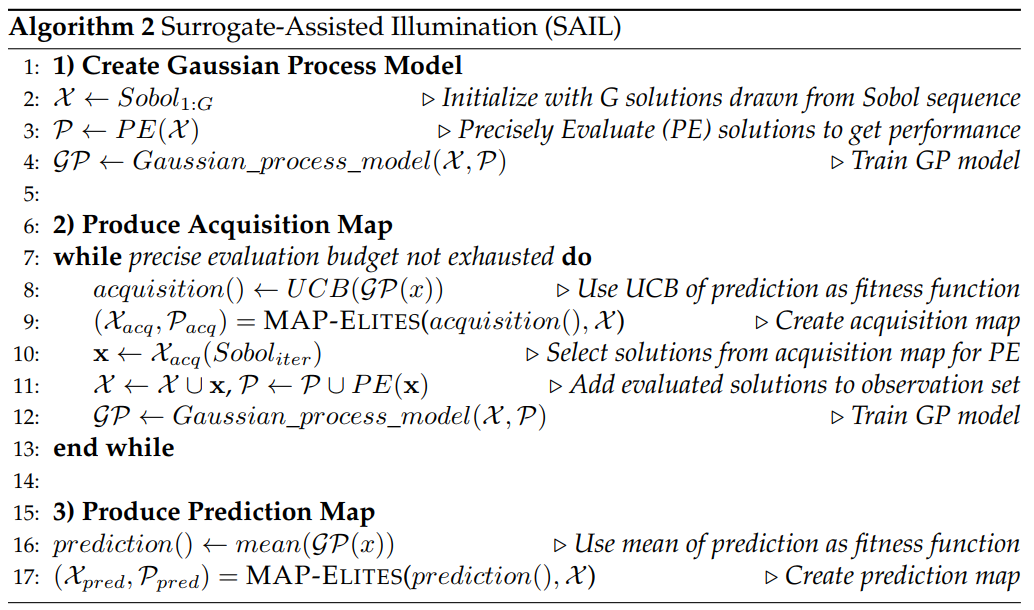
\psfig{file=SAILpcode.PNG,width = 4in}
%\caption{}
%\label{fig:SAILpcode}
%\end{figure}

\begin{algorithm}[h]
\DontPrintSemicolon
\SetAlgoLined
    \SetKw{thing}{1) Create Gaussian Process Model}
    \thing{}
    
    $\mathcal{X}\leftarrow Rand_{1:G}$ 
    
    %\tcp{Initialize with G random individuals}
    
    $\mathcal{P}\leftarrow PE(\mathcal{X})$ %\tcp{Precisely evaluate individuals}
    
    $\mathcal{G}\mathcal{P}\leftarrow Gaussian_process(\mathcal{X},\mathcal{P})$
    %\tcp{Train GP}
    
    \SetKw{secondStage}{2) Produce Acquisition Map}
    \secondStage{}
    
    \While{precise evaluation budget not exhausted}{
        $acquisition()\leftarrow UCB(\mathcal{G}\mathcal{P}(x))$
        
        %\tcp{Create acquisition function}
        
        $(\mathcal{X}_{acq}, \mathcal{P}_{acq}) = $ MAP-Elites $(acquisition(), \mathcal{X})$
        
        %\tcp{Illuminate acquisition function}
        
        $x\leftarrow \mathcal{X}_{acq}(Rand)$
        
        %\tcp{Select individuals from acquisition map}
        
        $\mathcal{X}\leftarrow \mathcal{X} \cup x, \mathcal{P}\leftarrow\mathcal{P} \cup PE(x)$
        
        $\mathcal{GP}\leftarrow Gaussian_process(\mathcal{X},\mathcal{P})$
    }
    
    \SetKw{thirdStage}{3) Produce Prediction Map}
    \thirdStage{}
    
    $prediction()\leftarrow mean(\mathcal{GP}(x))$
    
    $(\mathcal{X}_{pred},\mathcal{P}_{pred})=$ MAP-Elites $(prediction(),\mathcal{X})$
    
\caption{Surrogate Assisted Illumination (SAIL)\label{SAIL}}
\end{algorithm}

The first stage of the algorithm consists of sampling the problem space and building a Gaussian processes that will model fitness.
Recalling the foil terminology used in section 3.1, SAIL would create random individuals with \textit{M} and \textit{P} values, compute the precise model for each of them, and use those results to build a Gaussian process.

The second stage of SAIL trains the Gaussian processes by producing an \textit{acquisition map}.
Here, an acquisition function is computed from the Gaussian process using the \textit{Upper Confidence Bound} (UCB).
It is important to note that even though UCB is a linear combination of components, these components are in no way simple shapes.
For this reason, the acquisition function will not have an intuitive shape either.
Moreover, the acquisition function reflects the dimensionality of the feature space.
In a high dimensional feature space, the aquisition function will be a complicated high dimensional function.
Considering this, finding optima in the acquisition function can become a challenge.
MAP-Elites is perfectly suited to find not just the global optima of the acquisition function, but illuminate the acquisition function across the entire feature space.
The resulting set of high utility individuals is called the \textit{acquisition map}. 

SAIL takes a random set of individuals from the acquisition map, and runs the computationally expensive model on them.
Now there is a larger set of observed values that can be used to retrain the Gaussian processes.
The loop will enter its next iteration, repeating the process of creating the acquisition function, illuminating the acquisition function to create an acquisition map, selecting individuals from the acquisition map for precise evaluation, and rebuilding the Gaussian process with the new observations.
This processes will continue until a fixed computational budget is reached.

Through extensive iteration, the Gaussian process solidifies into a robust model that accurately describes the underlying function.
The goal of SAIL is to illuminate the underlying function.
This task is fulfilled in the third stage of SAIL by illuminating the mean prediction of the Gaussian processes using MAP-Elites.
The result of this illumination is a set of well performing solutions describing the various optima of the problem space.
We call this resulting set of solutions the prediction map.

\section{3D Foil Experiment: Velomobile Experiment}
\label{3DFoilExperiment}

Gaier et al included two experiments in their paper.
Due to space constraints, we will only visit the more ambitious of the two:
The application of SAIL to design three dimensional shapes of aerodynamic hulls for \textit{velomobiles}.
Velomobiles, shown in Figure \ref{fig:Velomobile}, are fully human powered ``bicycles''.
The cyclists in a velomobile sit in a \textit{recumbent position}, like one would sit in a paddle boat, and are enclosed in an aerodynamic hull.
The hull allows engineers to carefully craft the airflow around the velomobile to reduce drag.
Beause of this reduced drag, velomobiles hold several world speed records for human powered devices.

\begin{figure}[htb]
\centering
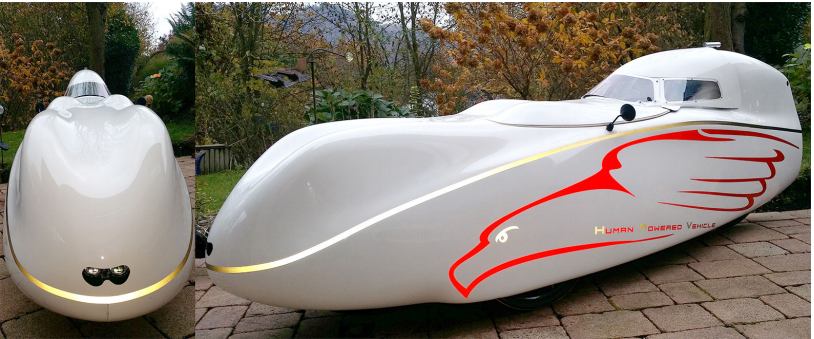
\psfig{file=Velomobile.PNG,width = 3in}
\caption{Milan Velomobile. Taken from \cite{Gaier:2018}}
\label{fig:Velomobile}
\end{figure}

Figure \ref{fig:Velomobile} shows how velomobiles have unintuitive hull shapes.
The strange contours to these hulls provide an interesting problem space to illuminate.
Moreover, the fluid dynamics software that simulates how air moves around the hull shape has high computational cost, stressing the need for a \textit{data efficient} approach to illumination.
In short, the illumination of velomobile hulls is a good testing ground for SAIL.

Gaier et al encountered several difficulties with this experiment.
Most prevalently, the data efficient nature of this problem rules out use of MAP-Elites as a control.
With MAP-Elite's heavy reliance on the computationally expensive model, illuminating these shapes would take hundreds, if not thousands of hours.
Previous experiments in \cite{Gaier:2018} demonstrate SAIL's ability to create near optimal solutions in fluid dynamic contexts, so the focus shifted from testing SAIL's ability to compete against other illumination algorithms, to focusing on how different velomobile representations affect performance of the SAIL algorithm.
Two representations, or encodings, of velomobile shape, are used in this experiment: a parameterized, and deformed encoding.

\subsection{Parameterized Encodings}
The parameterized encoding uses a set of aerofoil shapes to create a three dimensional velomobile hull as seen in Figure~\ref{fig:ParameterizedEncoding}.

\begin{figure}[htb]
\centering
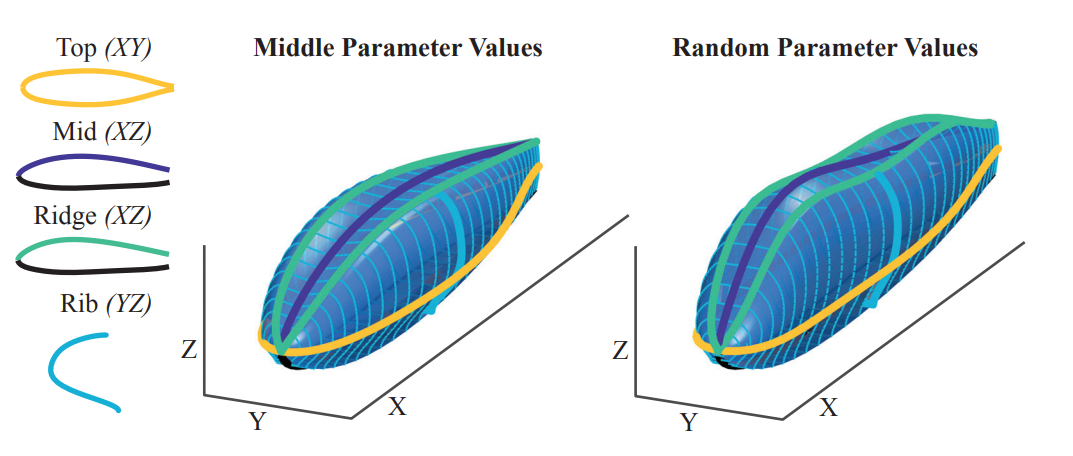
\psfig{file=ParameterizedEncoding.PNG,width = 3in}
\caption{Parameterized Encoding. Taken from \cite{Gaier:2018}}
\label{fig:ParameterizedEncoding}
\end{figure}

There are four foil shapes in the parameterized encoding.
The top foil shape, a symmetrical foil, defines the hull at its widest point from above.
The mid foil shape represents the foil at it's centerline.
The ridge foil represents the hull where the cyclist's knees protrude upward.
Finally, the rib foil affects how aggressively curved the surface of the hull will be.
All in all, this encoding will contain 16 parameters. 
An advantage of an encoding like this is that each of the 16 parameters directly change the aerodynamic properties of their respective foil shapes.

\subsection{Deformation Encodings}
Where the parameterized encoding represent key aspects of the shape directly relating to performance, deformed encodings take another approach.
Deformation encodings ``decouple the complexity of a the design from the complexity of the representation''\cite{Gaier:2018}.
That is, these encodings allow SAIL to find key features of foil performance on its own.
Figure \ref{fig:Deformation} shows an example of a deformation encoding:

\begin{figure}[htb]
\centering
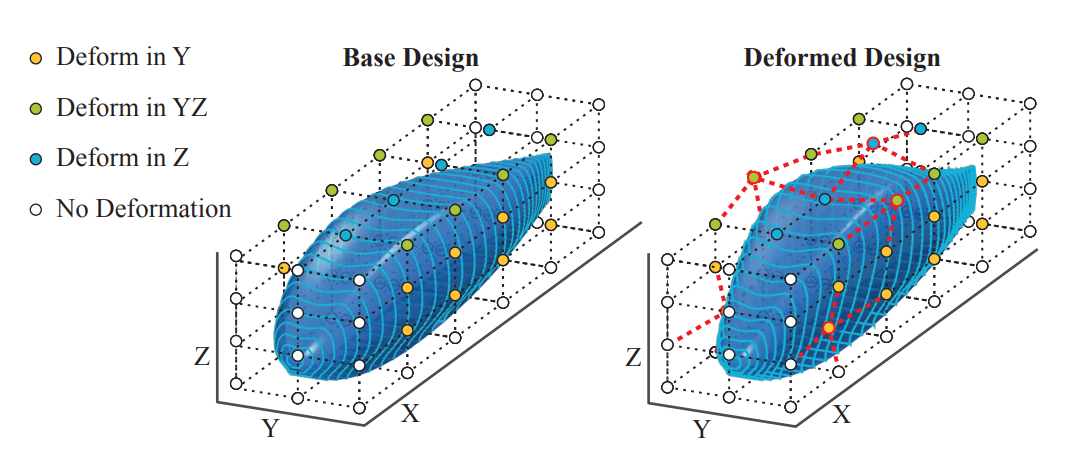
\psfig{file=Deformation.PNG,width = 3in}
\caption{Deformed Encoding. Taken from \cite{Gaier:2018}}
\label{fig:Deformation}
\end{figure}

Deformation encodings start with a base design, and surround it with a \textit{lattice}, or grid, of \textit{control points}.
These control points can be shifted in a particular axis.
As a control point is moved, the base design will \textit{deform} to adjust to the shifted control point.
Gaier et al allow  16 different points to be altered, each in only one axis.

\subsection{Experimental Setup}
The goal of this experiment is to see how two features, curvature and volume, impact the drag of a velomobile shape.
It is known that an increase in volume leads to an increase in drag, but a designer might want to explore how volume impacts drag to accommodate shifting requirements regarding volume (the pedaling mechanism requiring more space).
Moreover, designs with less curvature generally have less drag, but the thin carbon fiber might require additional (heavy) reinforcement to prevent flutter at high speed. 

SAIL started with 200 velomobile shapes to train the GP. During each iteration of the illumination phase, 10 individuals were chosen from the acquisition map to improve the GP.
There were a total of 100 illumination iterations leading to $200 + 10*100=1200$ precise evaluations during the illumination phase.
The feature map was discretized into a 25 x 25 map, leading to 625 bins. 

Fitness was computed as the drag force on the velomobile as it travels at 20 m/s (44.7 mph).
A low drag force will represent a better velomobile.

\subsection{Results: Design Performance}
Figure \ref{fig:DesignPerformance} shows the prediction maps for both the deformed and parameterized encodings as well as a comparison against the two.
In the left two images, a lighter colour indicates more drag, and a cooler colour indicates less.
We are aiming to minimize drag, so darker regions are preferred.

\begin{figure}[htb]
\centering
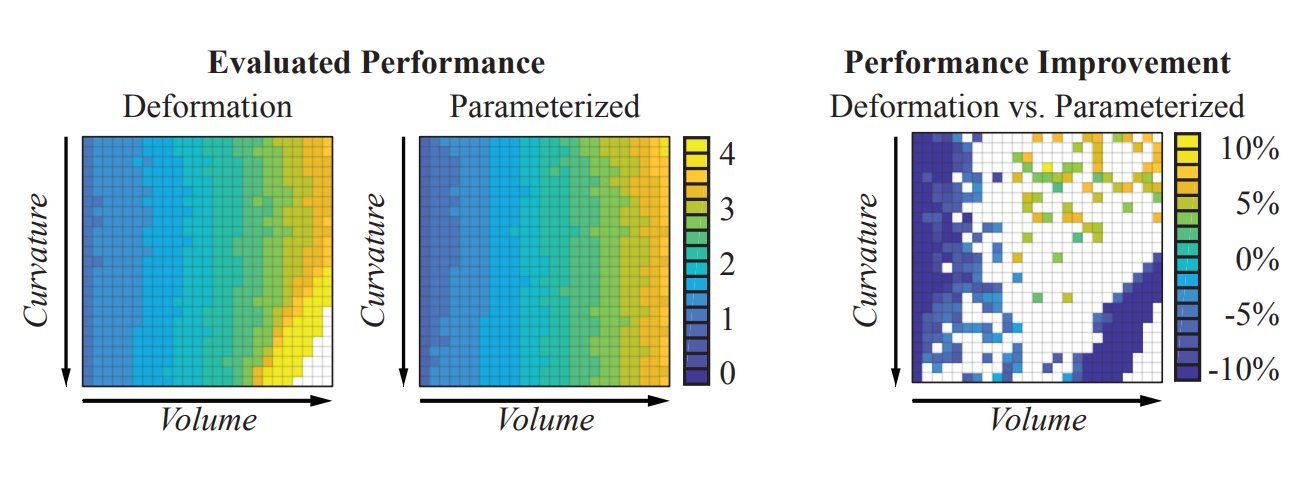
\psfig{file=DesignPerformance.png,width = 3in}
\caption{(Left) Prediction maps from deformed and perameterized encodings. (Right) Comparison of the two encodings. Taken from \cite{Gaier:2018}}
\label{fig:DesignPerformance}
\end{figure}

The deformation encoding has a set of empty bins in the high volume, high curvature section of its prediction map.
This is because the deformed encoding is too tightly constrained to create high volume, high curvature solutions.
It's clear that drag does increase with volume.
Encoding constraints aside, curvature does not seem to impact on drag.

The right side of Figure \ref{fig:DesignPerformance} shows the deformation encodings' successes against the parameterized encoding.
Lighter colour highlights regions where deformation has a better fitness than the parameterized encoding;
cooler colour indicates the converse.
There is only colour where there is a significant change in fitness between the two encodings.
Deformation does better in the high volume, low curvature region of the feature space, where as the parameterized encoding does better around the edges of the feature space.

\subsection{Results: Model Accuracy}
After each run, the individuals in the prediction map where precisely evaluated in order to record errors in the final GP model.
Figure \ref{fig:ModelAccuracy} shows that roughly 60\% of the drag calculations for individual's where within 5\% of the computationally expensive model.
The left side of Figure \ref{fig:ModelAccuracy} shows the deformed encoding has slightly lower error than the parameterized encoding.
However, it's unclear why.

\begin{figure}[htb]
\centering
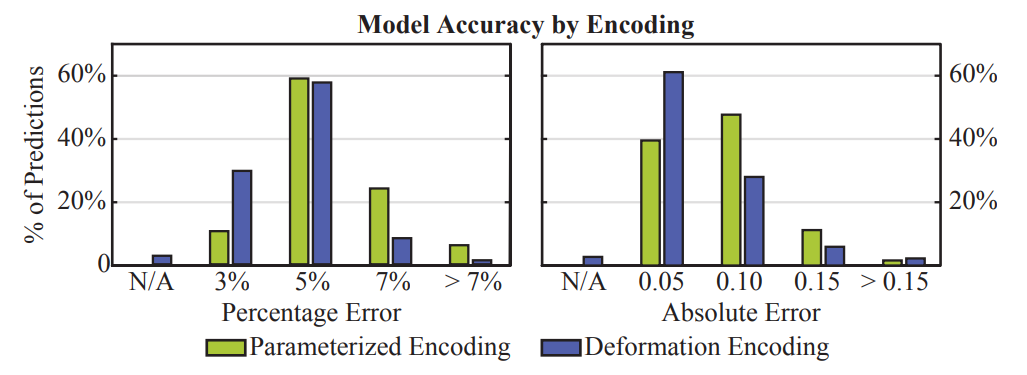
\psfig{file=ModelAccuracy.PNG,width = 3in}
\caption{GP error for both encodings. From \cite{Gaier:2018}}
\label{fig:ModelAccuracy}
\end{figure}

\subsection{Results: Design Exploration}
The two encodings lead to very different looking solutions that occupy the same bins in the prediction map at the end of the SAIL run.
Figure \ref{fig:3DShapes} shows two sets of similarly performing solutions (one of each encoding) that occupy the same bin.
Across the prediction map, the parameterized encoding is taller than its deformation analog.

\begin{figure}[htb]
\centering
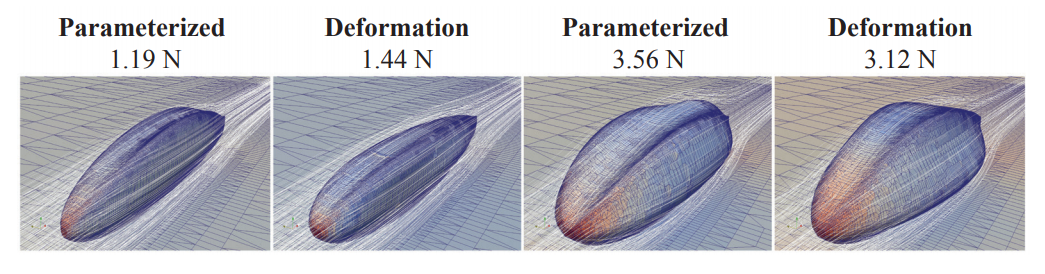
\psfig{file=3DShapes.PNG,width = 3in}
\caption{Two sets of similarly performing solutions that highlights the geometric tendencies of each encoding.
The left side includes two similarly performing low volume velombiles.
The right includes two similar high volume designs.
The red indicates how aerodynamic pressure is distributed over the velomobile shape.
Areas of greater intensity of red indicate higher aerodynamic pressure.
The numbers above the figures refer to drag force of the individual in \textit{newtons}.
Taken from \cite{Gaier:2018}}
\label{fig:3DShapes}
\end{figure}

Gaier et al suspect that parameterized encodings are taller than deformed encodings because they have more freedom to pinch the nose of the velomobile than deformed encodings can.
A pinched nose reduces frontal area, thereby reducing pressure on the nose of the velomobile.
While deformed designs lack this geometric freedom, they make up for it by smoothing out the shape along the length of the entire velomobile, especially where the ridges meet the hull.

These experiments show how various encodings can reach similarly performing solutions from different directions.
Moreover, they showcase SAIL's ability to create a variety of high performing solutions independent of encoding.

\section{Conclusions}
\label{sec:conclusions}
The velomobile experiment demonstrates several of SAIL's capabilities.
They show the potential of SAIL as a powerful algorithm for illuminating problem spaces in computationally difficult problem spaces.
Moreover, SAIL could be used for testing the limits of various encodings.
Before committing to a specific encoding, SAIL can show whether or not that encoding is capable of reaching far areas of the feature space.
Moreover, SAIL can give an engineer insights as to how each individual point of variation in the encoding contributes to performance. 

A particular advantage of SAIL is that it returns, not only a set of high performing solutions, but also the Gaussian proccess model.
This model can be used to gain additional insights into the problem space

Gaier et al mention that a potential bottleneck for SAIL is the behavior function.
For example, computing curvature for each velomobile precisely would be too computationally expensive.
The authors used a simplified model to compute curvature that was significantly faster.
Gaier et al propose the expanded use of surrogate models in the behavior function in cases where the behavior function is too computationally expensive to run for every individual in a SAIL run.

\section*{Acknowledgments}
There are many people who deserve acknowledgment for the help they have provided me during this senior seminar. Thank you to Andrew Kroska, Islamzhan Saliyev, and Kirbie Dramdahl for their gracious time, and review of this paper.
Thank you to my advisor, Dr. Nic McPhee, for his continued mentorship and time throughout this semester and my college career.
Thank you to the Computer Science faculty at University of Minnesota Morris.
Finally, thank you to Alexa Barta for her continued support.
\label{sec:acknowledgments}

% The following two commands are all you need in the
% initial runs of your .tex file to
% produce the bibliography for the citations in your paper.
\bibliographystyle{abbrv}
% sample_paper.bib is the name of the BibTex file containing the
% bibliography entries. Note that you *don't* include the .bib ending here.
\bibliography{sample_paper}  
% You must have a proper ".bib" file
%  and remember to run:
% latex bibtex latex latex
% to resolve all references

\end{document}
